\section{Usar complementos}\index{plugins}

\subsection{Una introducción al uso de complementos}\label{label_introplugin}

QGIS se ha diseñado con una arquitectura de complementos. Esto permite que se añadan nuevas funciones a la aplicación. Muchas de las funciones actuales de QGIS están en realidad implementadas como complementos.

Hay dos tipos de complementos en QGIS: integrados o aportados por usuarios. \index{plugins!types} Un complemento integrado es mantenido por el equipo de desarrollo de QGIS y forma parte de cada distribución de QGIS. Un complemento aportado por usuarios es un complemento externo que es mantenido por el autor individual. La web del SVN de QGIS (\url{http://svn.qgis.org}) sirve algunos complementos aportados por usuarios.

\subsubsection{Encontrar e instalar un complemento}
Cuando instala QGIS, todos los complementos integrados están incluidos (vea el capítulo \ref{sec:core_plugins}). \index{plugins!installing}
% Additional user-contributed
% plugins may be available on the QGIS Community site. To see what
% user-contributed plugins are available, see the plugins page on the Community
% site (\url{http://community.qgis.org/plugins}).\index{plugins!user
% contributed}

De forma típica, los complementos aportado por usuarios se distribuyen en forma de código fuente y hay que compilarlos. Para instrucciones sobre la compilación e instalación de un complemento aportado por usuarios, vea la documentación incluida con el complemento.

\subsubsection{Administrar complementos}\label{sec:managing_plugins}
\index{plugins!managing} La administración de complementos consiste en cargarlos o descargarlos desdes QGIS. Los complementos cargados se «recuerdan» cuando sale de la aplicación y son restaurados la siguiente vez que ejecuta  QGIS.

Para administrar complementos, abra el \textsl{Administrador de complementos} desde el menú \textsl{Complementos}. \index{plugins!manager}El Administrador de complementos muestra todos los complementos disponibles y su estado (cargados o no cargados). La Figura \ref{fig:pluginmanager} muestra el diálogo del Administrador de complementos.

\begin{figure}[ht]
   \begin{center}
   \caption{Administador de complementos}\label{fig:pluginmanager}\smallskip
   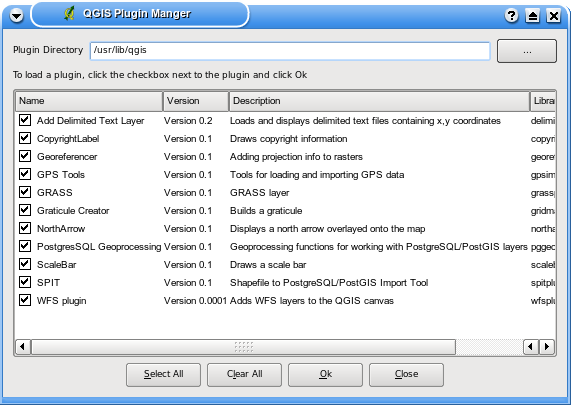
\includegraphics[clip=true, width=14cm]{pluginmanager2}
\end{center}  
\end{figure}

De forma típica todos los complementos de QGIS se instalan en la misma ubicación. Esta localización se muestra en el campo de texto Directorio de complementos. Le puede decir a QGIS que cargue complementos desde otra localización especificando un directorio distinto.

\begin{Tip}\caption{\textsc{Complementos que se cuelgan}}\index{crashes}
\qgistip{Si nota que QGIS se cuelga al iniciar, puede que haya un complemento que está dando problemas. Puede detener todos los complementos para que no se carguen editando su archivo de configuración guardado (vea \ref{subsec:gui_options} para su localización). Localice la configuración de los complementos y cambie todos los valores a false para evitar que se carguen. Por ejemplo, para evitar que se cargue el complemento Texto delimitado, la entrada en \$HOME/.config/QuantumGIS/qgis.conf en Linux debería ser como esta::\ttfamily{Add Delimited Text Layer=false}.\normalfont Haga esto con cada  complemento en la sección [Plugins]. Luego puede arrancar QGIS y añadir los complementos de uno en uno desde el Administrador de complementos para determinar cuál está ocasionando los problemas.
}
\end{Tip} 

\subsubsection{Proveedores de datos}\index{data providers}

Los proveedores de datos son complementos «especiales» que proporcionan acceso a un almacén de datos. De forma predeterminada, QGIS soporta capas PostGIS y almacenes de datos basados en disco soportados por la biblioteca GDAL/OGR (Apéndice \ref{appdx_ogr}). Un complemento de proveedor de datos amplía la capacidad de QGIS para usar otras fuentes de datos.

Los complementos de proveedores de datos son registrados automáticamente por QGIS al iniciarse. No son gestionados por el Administrador de complementos, pero se usan sin notarlo cuando el tipo de datos correspondiente se añade como capa en QGIS.

\subsubsection{Complementos integrados}\label{sec:core_plugins}\index{plugins!core}

Actualmente QGIS contiene 9 complementos integrados que se pueden cargar usando el Administrador de complementos. La tabla \ref{tab:core_plugins} lista cada uno de los complementos integrados junto con una descripción de su propósito y el icono de la barra de herramientas. Note que el complemento de GRASS no está incluido abajo, porque éste instala su propia barra de herramientas (vea la sección \ref{sec:grass} para ver en detalle las funciones disponibles en el complemento de GRASS).

% minipage is needed to appear the footnote under the table
% SH
\begin{minipage}{\textwidth}
\begin{table}[H]
\centering
\caption{QGIS Core Plugins}\label{tab:core_plugins}\medskip
\small
 \begin{tabular}{|l|l|p{4in}|}
\hline \textbf{Icon} & \textbf{Plugin} & \textbf{Description} \\
\hline 

\includegraphics[width=0.7cm]{copyright} & Copyright Label \index{plugins!copyright}& Display a copyright label on the map canvas\\
\hline 

\includegraphics[width=0.7cm]{delim_text} & Delimited Text \index{plugins!delimited text}& Load a delimited text file containing x,y coordinates as a point layer \\
\hline 

\includegraphics[width=0.7cm]{gps} & GPS Tools \index{plugins!gps}& Load and display GPS data \\
\hline 
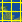
\includegraphics[width=0.7cm]{gridmaker} & Graticule Creator \index{plugins!graticule}& Create a latitude/longitude grid and save as a shapefile\\
\hline 

\includegraphics[width=0.7cm]{scalebar} & Scalebar \index{plugins!scalebar}& Add a scalebar to the map canvas\\
\hline 

\includegraphics[width=0.7cm]{northarrow}& North Arrow \index{plugins!north arrow}& Add a north arrow to the map canvas\\
\hline 
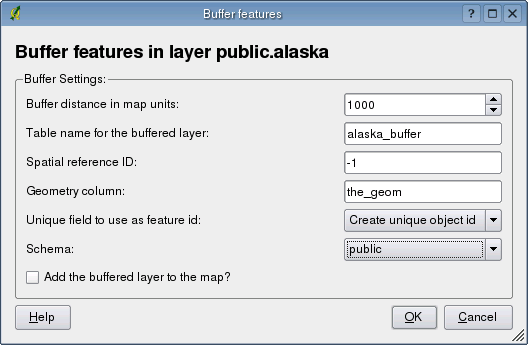
\includegraphics[width=0.7cm]{buffer} & PostgreSQL Geoprocessing \index{plugins!geoprocessing}& Buffer a PostGIS layer \\
\hline 

\includegraphics[width=0.7cm]{spiticon} & SPIT \index{plugins!SPIT}& Shapefile to PostGIS Import Tool - import shapefiles into PostgreSQL\\
\hline
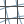
\includegraphics[width=0.7cm]{georeferencer} & Georeferencer\footnote{The georeferencer-plugin is only available if you have installed the gsl-libraries and headers during compile-time. Please check the installation-chapter \ref{sec:install_gsl} for details.} \index{plugin!Georeferencer} & Georeferencing rasterlayers \\
\hline

\includegraphics[width=0.7cm]{wfs-icon} & WFS & Load and display WFS layer \\
\hline
\end{tabular}
\end{table}
\end{minipage}

\normalsize


\begin{Tip}\caption{\textsc{Plugins Settings Saved to Project}}\index{plugins
settings}
\qgistip{When you save a .qgs project, any changes you have made to
NorthArrow, ScaleBar and Copyright plugins will be saved in the project and
restored next time you load the project.
}
\end{Tip}

%
% External Plugins
%
\subsubsection{External Plugins}\label{sec:external_plugins}\index{plugins!external}

QGIS also comes with some externally developed plugins. They are not shipped with the
default distribution. However, they can be compiled and used within QGIS.

Currently the external plugins are only available directly from SVN. 
To check out all available external plugins do the following:
\begin{verbatim}
svn co https://svn.qgis.org/repos/qgis/trunk/external_plugins external_qgis_plugins
\end{verbatim}

This will create a folder \texttt{external\_qgis\_plugins} in your current folder.
Each subdirectory has its own compile and install instructions. Read them carefully
in order to build the plugin.

%
% Plugin template
%
\subsubsection{Plugin templates}\label{sec:plugin_template}\index{plugins!template}

If you like to develop your own QGIS-plugin the main sources include a nice script
which guides you through the process of creating your own template-directory-structure
within the QGIS-source-tree.
The script lives in \texttt{QGIS/src/plugins/plugin\_builder.pl}.

The only thing to do is coding your functions into the plugin (and of course contribute
your plugin the the QGIS-development-team).

Beside that the QGIS-wiki (\url{http://wiki.qgis.org}) and the QGIS-blog (\url{http://blog.qgis.org})
provide useful articles about writing your own plugin as well.
Check the websites for details!
